\chapter{Isomorfní přístup k programování webových aplikací}
\label{sec:isomorphic}
Při startu nového projektu je v první řadě nutné navrhnout vhodnou architekturu a s ní související technologická řešení. U větších projektů se dnes stále častěji uvažuje o architektuře jednostránkových aplikací, které jsou dnes velmi populární. Mají ovšem několik podstatných nevýhod, jednou z hlavních je špatná indexovatelnost vyhledávači, jež je nevýhoda, která přímo vyplývá z návrhu, je tedy velmi těžké jí odstranit. Roboti internetových vyhledáváčů totiž většinou neovládájí Javascript a nedokážkou proto webové aplikace korektně zobrazit. Další nevýhodou běžných SPA je náročnost javascriptového kodu celé aplikace pro webový prohlížeč v mobilním telefonu, načítání jednostránkových aplikací často trvá příliš dlouho, což kazí celkový dojem uživatele \cite{spa} \cite{spa_book}. 

Mnohé z těchto nevýhod řeší takzvaný isomorfní přístup, který v oblasti programování webových aplikací znamená použití stejného programovacího jazyka pro backend\footnote{serverová část aplikace} i frontend\footnote{klientská část aplikace (webový prohlížeč)}. Poprvé s tímto pojmem přišel Charlie Robbins v roce 2011 ve svém článku \textit{Scaling Isomorphic Javascript Code} \cite{isomorphic_founder}, kde popisoval isomorfismus jako schopnost použití stejného kódu pro server i webový prohlížeč. Jediným jazykem, který lze dnes takto použít je Javascript. Tento přístup poté popularizoval Spike Brehm v roce 2013 v článku \textit{Isomorphic Javascript: The Future of Web Apps} \cite{isomorphic_airbnb2}.

Isomorfismus je obecně pojem pro zobrazení mezi dvěma matematickými strukturami, které je vzájemně jednoznačné a zachovává všechny vlastnosti touto strukturou definované. Jinými slovy, každému prvku první struktury odpovídá právě jeden prvek struktury druhé a toto přiřazení zachovává vztahy k ostatním prvkům \cite{isomorphic_def}. Pojem lze dobře vizualizovat pomocí grafů, na obrázku \hyperref[label:isomorphic_graph]{4.1} jsou dva vzájemně isomorfní grafy.

\begin{figure}[h]
\begin{centering}
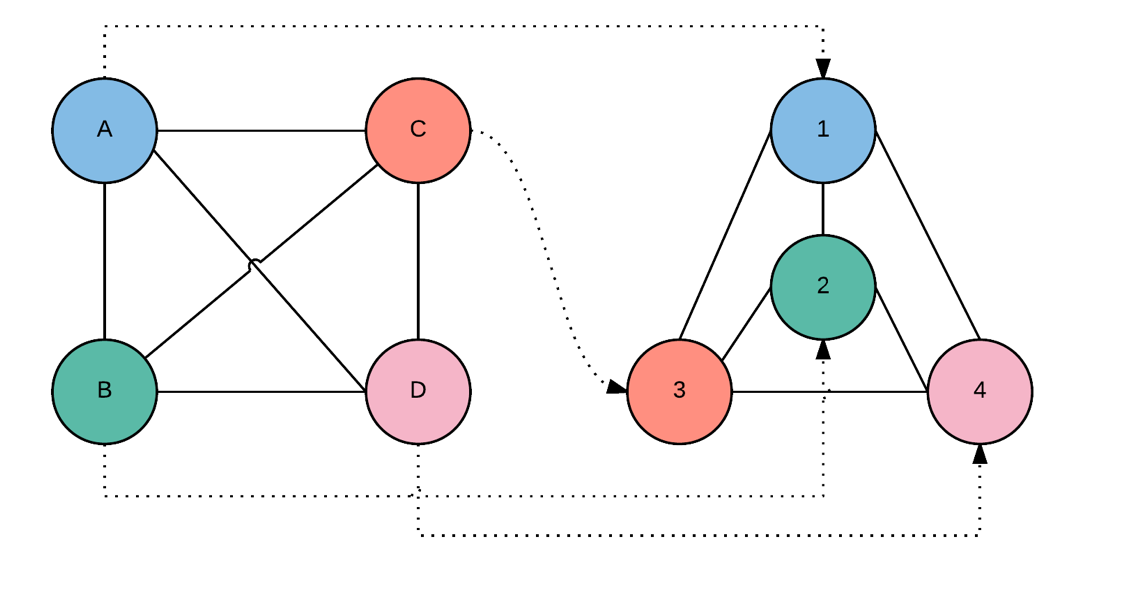
\includegraphics[scale=0.5]{obrazky/isomorphic_graph}
\par\end{centering}
\caption{Dva vzájemně isomorfní grafy \cite{isomorhic_book} \label{fig:isomorphic_graph}}
\end{figure}
\FloatBarrier

Isomorfní webová aplikace\footnote{V době dokončování této práce bylo komunitou rozhodnuto o používání názvu \textit{univerzální webové aplikace} \cite{universal_js}. V této práci se budu držet původního termínu isomorfní.} je ze své podstaty také jednostránkovou aplikací, která ovšem mnohem více zapojuje serverovou část. Ta je u klasických jednostránkových aplikací redukována na servisní vrstvu a datové API. Takto navržené aplikace používají stejný javascriptový kód pro webový prohlížeč i webový server, což má pro vývoj několik zajímavých důsledků \cite{isomorhic_book}:

\begin{itemize}
\item vývojáři udržují jen jeden hlavní projekt (codebase),
\item isomorfní web částečně funguje i bez Javascriptu,
\item možnost používání stejných knihoven pro server i prohlížeč.
\end{itemize}

Takto navržené webové aplikace začínají být velice populární. Příkladem je hlavně Facebook nebo třeba Airbnb \cite{isomorphic_airbnb} \cite{isomorphic_airbnb2}, Netflix \cite{netflix} nebo nová verze Uber. Dnes existuje mnoho knihoven pro vývoj isomorfních webových aplikací, některé z nich vznikly ve společnosti Facebook, jako výsledek složitého vývoje sociální sítě. Nejzásadnější z nich, framework React přinesl zcela nový pohled na návrh a implementaci uživatelských rozhraní. Také oblíbená architektura Flux, která přináší sjednocení práce s daty aplikace, vznikla ve stejné společnosti \cite{flux}. Mnoho existujících javascriptových knihoven pro prohlížeč jako Underscore, Backbone.js, Handlebars.js, Moment nebo jQuery, je možné používat také na serveru s nulovými nebo minimálními úpravami \cite{isomorphic_airbnb2}.

\section{Výhody isomorfního přístupu}
Isomorfní přístup k programování webových aplikací je výsledek více než dvaceti let evoluce v tomto oboru. Princip využívá interaktivity a uživatelské přívětivosti klasických jednostránkových webových aplikací v Javascriptu, které rozšířuje a vylepšuje pomocí většího zapojení serveru. Isomorfní přístup také řeší většinu nevýhod klasických webových aplikací. Například díky možnosti vykreslování šablon na straně serveru řeší problém indexace běžných SPA. Vyhledávací robot bez Javascriptu uvidí stejný web jako běžný uživatel s Javascriptem \cite{isomorhic_book}. Následující kapitola popíše hlavní výhody isomorfismu spolu s řešením častých problémů jednostránkových webových aplikací.

\subsection{Sjednocení používaného jazyka a prostředí}
První a nejdůležitější výhodou a sjednocení používaného jazyka, jinými slovy možnost použití Javascriptu pro prohlížeč i server. Isomorfní aplikace kvůli principu sdílení kódu zpravidla používají dokonce jeden projekt pro obě prostředí. Vždy ale bude existovat nějaká logika určená jen pro prohlížeč nebo jen pro server. Podle doporučovaných konvencí je proto vhodná rozdělit isomorfní aplikaci na tři základní adresáře: \textit{client}, obsahující kód pouze pro prohlížeč, \textit{server} s kódem určeným pro server a \textit{common}, který obsahuje sdílený kód \cite{isomorhic_book}.

Dva následující obrázky dobře ilustrují rozdíly mezi architekturami běžných a isomorfních SPA \cite{codepicnic_universaljs}.
\begin{figure}[h]
\begin{centering}
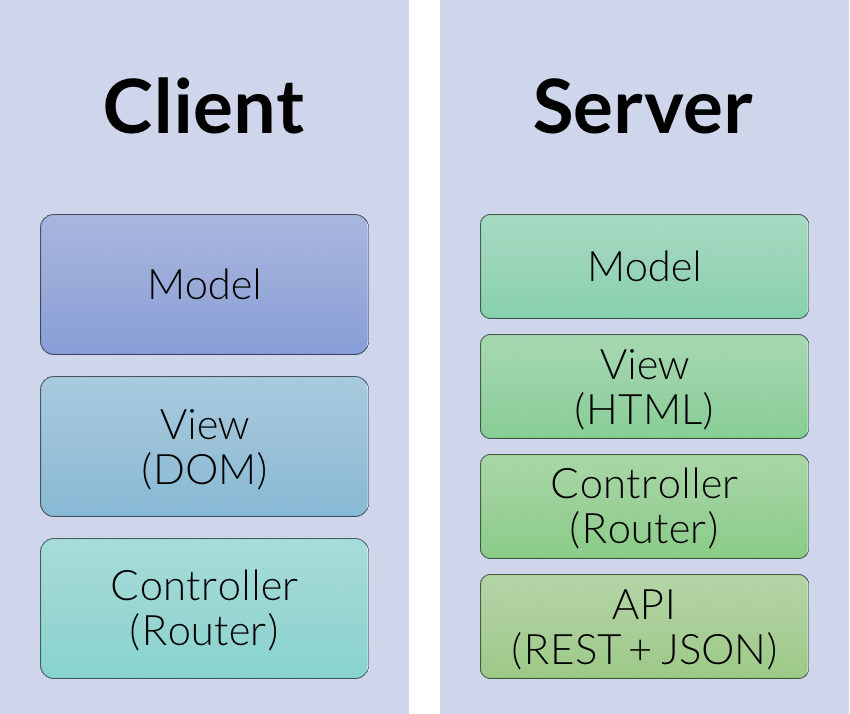
\includegraphics[scale=0.5]{obrazky/classic_webpage_architecture}
\par\end{centering}
\caption{Diagram architektury typické jednostránkové webové aplikace \cite{codepicnic_universaljs} \label{fig:classic-web-arch-diagram}}
\end{figure}

Jak je vidět na diagramu výše, SPA podle původního konceptu přesunulo většinu zodpovědnosti z serveru na klienta, uvnitř webového prohlížeče probíhá vykreslování šablon, routování požadavků a další věci, které dříve vždy řešil server. Při vzniku SPA to bylo považováno za výhodu, díky snížení nároků na webové servery \cite{spa_book}. Redukce serverové části aplikace na datové API však přinesla také mnohé nevýhody, jednostránková aplikace byla mnohem výpočetně náročnější než běžná webové aplikace, indexovatelnost a obecně SEO bylo problémem. Po několika letech boomu jednostránkových aplikací se tak začaly objevovat názory, že je nutné některé věci přesunout zpět na webový server. V této době byla již velmi používaná platforma node.js, bylo tedy možné napsat i serverovou část aplikace v Javascriptu a tím používat stejný jazyk pro obě prostředí. Isomorfní webová aplikace tedy používá pouze jazyk Javascript, pro klient i server. Typicky serverové problémy, jako vykreslování šablon nebo routování požadavků byly přesunuty zpět na na stranu serveru \cite{isomorhic_book}.
\begin{figure}[h]
\begin{centering}
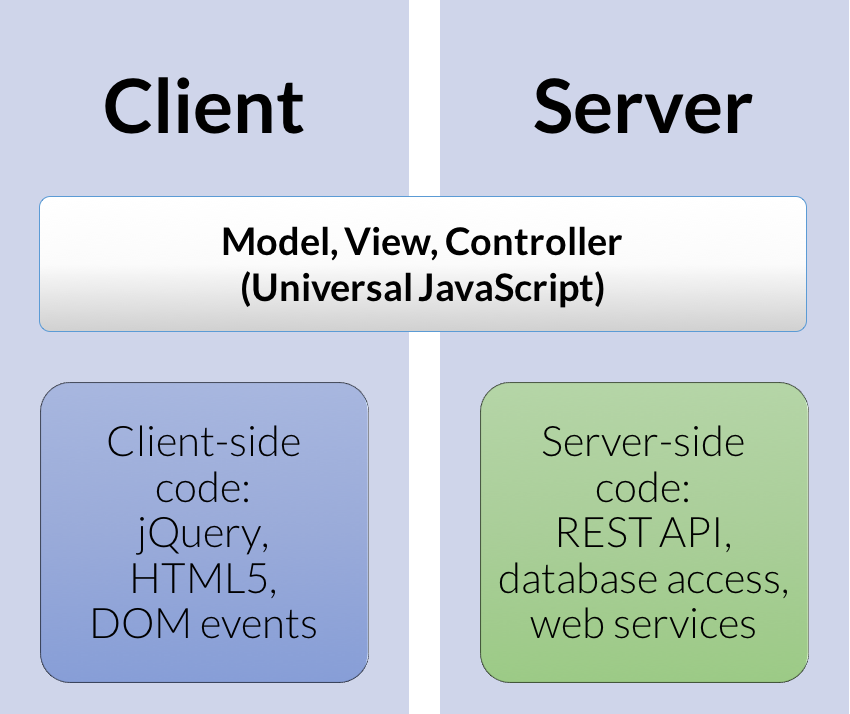
\includegraphics[scale=0.5]{obrazky/isomophic_webpage_architecture}
\par\end{centering}
\caption{Diagram architektury isomorfní webové aplikace \cite{codepicnic_universaljs} \label{fig:isomophic-web-arch-diagram}}
\end{figure}
\FloatBarrier

\subsection{Interaktivita jednostránkových aplikací}
I isomorfní webová aplikace je pořád jednostránkovou webovou aplikací, se všemi jejími výhodami. Veškeré interakce s uživatelem probíhají asynchronně bez dalšího načítání nové stránky. Server řídí routování požadavků a vykreslování stránek a to buď přímo při prvním načtení aplikace nebo pomocí AJAX při procházení navigace. Koncept isomorfních webových aplikací vylepšuje koncept SPA rozšířením kompetencí webového serveru a zároveň tím řeší největší problémy jednostránkových webových aplikací \cite{isomorhic_book}.

\subsection{Sdílení kódu mezi prostředími}
Obvykle nejčastěji zmiňovanou výhodou isomorfních webových aplikací je možnost sdílení zdrojového kódu. Možnost sdílení kódu mezi prohlížečem a serverem přináší určitá specifika, na které je nutné při vývoji isomorfních webových aplikací myslet. Zejména je nutné vyhnout se používání rozhraní, které je specifické pro dané běhové prostředí, například objekt \textit{window} v prohlížeči, nebo \textit{env} v node.js. Místo toho je nutné používat obslužné metody isomorfního frameworku, který zapouzdřuje tyto specifická rozhraní a umí je dle prostředí přízpůsobit. Tento přístup je nazývá \textit{environent-agnostic} a definuje tvorbu univerzálně použitelného Javascriptu, který správně funguje na všech prostředích \cite{isomorhic_book} \cite{codepicnic_universaljs}.

Je tedy možné sdílet mnoho použitého kódu, například šablony nebo validační pravidla, některé části aplikace, jako například router, je ale nutné implementovat zvlášť pro server a pro prohlížeč. Části, které je nutné zdvojit, však většinou není nutné udržovat na dvou místech, moderní isomorfní devstacky dokážou tyto procesy automatizovat. Například u routovacích pravidel se použitý task runner při spuštění aplikace postará o distribuci pravidel do serverového i klientského routeru \cite{isomorhic_book} \cite{codepicnic_universaljs}.

\vspace{3mm}
\noindent Následující ukázka kódu ilustruje implementaci funkce suma pro webový prohlížeč, server v node.js a její univerzální variantu. Ta používá IIFE (viz. \hyperref[sec:variable_scope]{2.2.2}), jež dostane jako parametr nejvyšší globální objekt daného prostředí. Tedy \textit{window} v případě prohlížeče a \textit{exports} v případě node.js.
\begin{lstlisting}[language=Javascript,caption={Ukázka principu enviroment-agnostic, tedy JS kódu nezávislého na běhovém prostředí}]
// Javascript v prohlížeči
function browserSum(a,b){
		return a+b;
}

// node.js
module.exports.serverSum = function(a,b){
		return a+b;
};

// univerzální Javascript (environment-agnostic)
(function(exports){
     exports.isomorphicSum = function(a,b){
     		return a+b;
     };
})(typeof exports ? exports : window);
\end{lstlisting}

Při použití vhodných nástrojů nemusí programátor nad nezávislostí kódu přemýšlet, řeší ji automaticky použitý framework. Také systém modulů, který přinesl Javascript ES6, pomáhá univerzálnosti javascriptového kódu.

\subsection{Rychlejší prvotní načtení aplikace}
Běžné jednostránkové aplikace se při prvním načtení kompletně nahrají do prohlížeče a spustí. Tohle prvotní načtení je ale většinou velmi náročné na zdroje i výpočetní výkon. Javascriptové jádro webové prohlížeče musí stáhnout a zpracovat všechny javascriptové soubory, načíst HTML šablony a celou aplikaci včetně všech dynamických prvků spustit. To může trvat i několik sekund. Server poskytuje jen čisté HTML, které většinou neobsahuje žádný text, ale jen definice všech zdrojů aplikace pomocí HTML značek \textit{script} nebo \textit{rel}. Naproti tomu isomorfní aplikace vrátí na první načtení již vykreslenou úvodní stránku, definice externích zdrojů jsou zastoupeny v mnohem menší míře, jelikož výpočetně náročné části řeší server \cite{isomorhic_book} \cite{codepicnic_universaljs}. Na následujícím grafu je dobře vidět rozdíl časů prvního načtení klasické jednostránkové aplikace postavené na velkém MVC frameworku a té využívající isomorfní přístup s pomocí frameworku React \cite{spa_perf}. 
\begin{figure}[h]
\begin{centering}
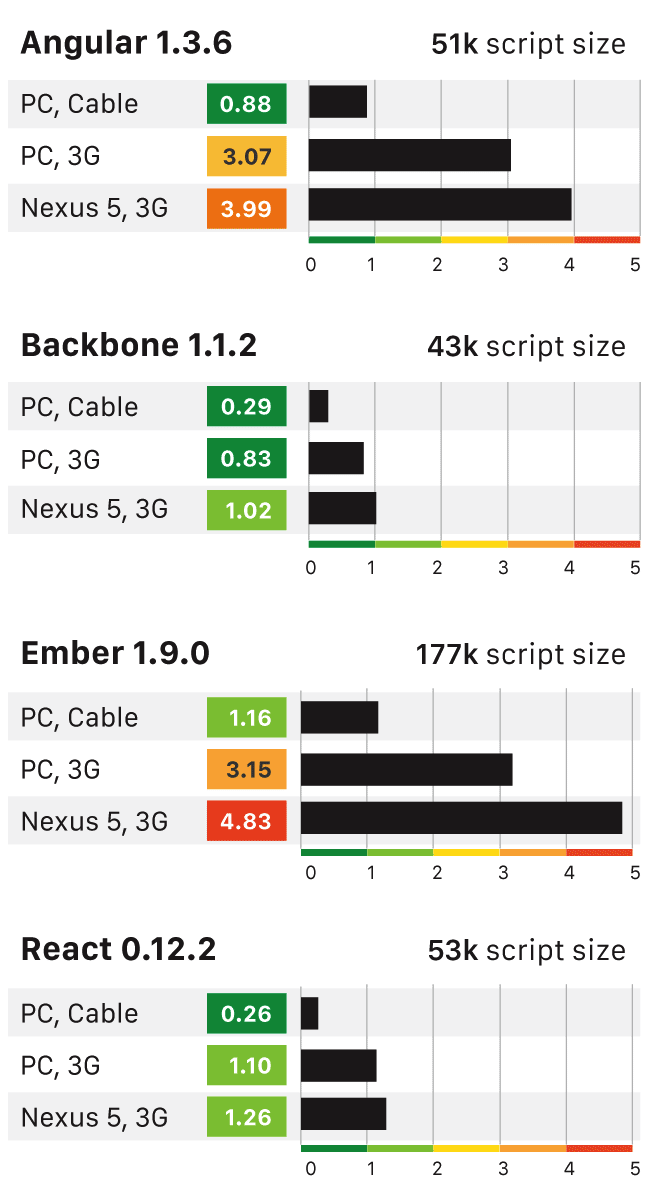
\includegraphics[scale=0.2]{obrazky/first_render_times}
\par\end{centering}
\caption{Graf časů prvotního načtení Javascriptových frameworků \cite{spa_perf} \label{fig:first_load_times}}
\end{figure}
\FloatBarrier

Jak je vidět, čas prvního načtení isomorfní aplikace využívající React je především díky serverovému vykreslování výrazně nižší. Také tolik nezáleží na výkonu koncového zařízení, isomorfní aplikace je stejně rychlá na mobilních telefonech jako v osobních počítačích \cite{isomorhic_book} \cite{codepicnic_universaljs}. 

\subsection{Indexovatelnost vyhledávači}
Známé javascriptové frameworky pro tvorbu běžných jednostránkových aplikací, jako například AngularJS, mají velký problém s indexovacími roboty vyhledávačů. Robot, který prochází Internet většinou nepodporuje Javascript, tím pádem se mu jednostránková aplikace, která plně běží v prohlížeči uživatele, nespustí. Vyhledávač potom nevidí strukturu ani obsah takové aplikace. Existuje několik řešení, pomocí kterých lze tento problém řešit. Jedna z možností je provozování celého webového prohlížeče uvnitř serveru v takzvaném headless (bezešvém) módu. Tento integrovaný prohlížeč potom zpracovává javacriptovou aplikaci na straně serveru a vyhledávacím robotům vrací kompletně vykreslenou stránku v čistém HTML, se kterou již indexační robot nemá nejmenší problém. Běžnjá isomorfní aplikace ale částečně vykresluje HTML na serveru, vyhledávácí roboti tak obdrží mnohem bohatší stránku než u klasických SPA. Tomuto přístupu se říká \textit{server-side rendering} \cite{isomorhic_book} \cite{codepicnic_universaljs}.

\subsection{Server-side rendering}
\label{sec:server_side_rendering}
Server-side rendering umožňuje vykreslovat javascriptové šablony na straně serveru a vracet je webovému prohlížeči už částečně zpracované. Tuto možnost přinesla platforma node.js, která je schopná používat většinu javascriptových frameworků, které jsou určeny pro prohlížeč. Díky tomu můžeme vykreslovat šablony na serveru naprosto ekvivalentně jako v prohlížeči, což je stěžejní část isomorfního přístupu. Ten používá server-side rendering jen při prvním načtení aplikace, další operace jsou již plně v režii webového prohlížeče. To znamená, že se stránka korektně zobrazí i vyhledávacím robotům nebo uživatelům s vypnutým Javascriptem. Server-side rendering tedy řeší jednu z často zmiňovaných nevýhod klasických jednostránkových aplikací. Tento přístup také podstatně zrychluje první načtení aplikace, není totiž nutné čekat na stažení a zpracování veškerého javascriptového kódu prohlížečem \cite{isomorhic_book} \cite{codepicnic_universaljs}.

\subsection{Vývoj mobilních aplikací}
Vzhledem k tomu, že je celá isomorfní aplikace naprogramována v Javascriptu, lze jí provozovat v každém webovém prohlížeči, včetně toho v mobilním telefonu. V mobilu lze webový prohlížeč spustit také bez uživatelského rozhraní (adresní řádek a podobně) a simulovat tím dojem nativní aplikace. Lze potom vyvíjet mobilní aplikaci v HTML, CSS a Javascriptu, která bude při správném nastylování prakticky k nerozpoznání od té nativní. Výhodou webových aplikací je nenáročnost na prostor, aplikace je včetně svých dat uložena na vzdáleném serveru, kde probíhají i některé výpočty. To usnadňuje také aktualizace, stačí pouze nahrát novou verzi na server. Pomocí frameworku Apache Cordova \cite{cordova}, je možné javascriptovou aplikaci distibuovat standardními prodejními kanály jako běžné aplikace. Zabalená aplikace jako první krok nastartuje webový prohlížeč mobilního zařízení a následně se v něm spustí. Aplikace je pak vytvořena jenom jednou a potom s drobnými úpravami vydána pro různé mobilní platformy. Některé frameworky podporující tvorbu mobilních aplikací v Javascriptu, poskytují také připravené grafické motivy, které reprezentují jednotlivé mobilní platformy. Stejné aplikace potom vypadá jinak na systému iOS a jinak na Androidu, vždy s ohledem na grafický styl dané platformy \cite{mobile_apps}. Tyto motivy nabízí například Ionic \cite{ionic}.

\section{Reaktivní programování}
Důležitým konceptem isomorfního přístupu je aplikování reaktivního programování. Jeho základním principem je vytváření celého uživatelského rozhraní znovu s každou provedou změnou. Dalším důležitým aspektem je princip komunikace pouze pomocí událostí. Každá změna dat musí být realizována pomocí této události. Ty jsou důležitou součástí reaktivního programování. Tento přístup dovoluje psát přehledné a dobře udržovatelné webové aplikace, protože se velmi zjednoduše datový model. Každá změna dat vždy vyvolá vytvoření nového modelu, na základě provedené změny a současného stavu. Aplikování reaktivního přístupu nad standartním Document Objekt Modelem je složité, protože jeho generování je velmi časové náročné \cite{isomorhic_book} \cite{codepicnic_universaljs}. Tento problém vyřešil až příchod mechanismu Virtual DOM, který přinesl framework React (viz \hyperref[sec:virtual_dom]{4.4.5}) \cite{virtualdom}.

\section{Imutabilní datové struktury}
\label{sec:immutability}
Další novinkou, která je v poslední době v Javascriptu populární, jsou imutabilní datové struktury. Jejich používání významně zrychluje celou webovou aplikaci. Podle definice imutabilita znamená \textit{neschopnost změny}, v programování se tak označují neměnné datové struktury, jejichž jakákoliv změna vždy vytvoří novou datovou instanci. Mutabilita potom znamená možnost změny a mutabilní je většina struktur v Javascriptu, některé, jako například pole, jsou imutabilní již nyní. S nástupem velkých javascriptových aplikací bylo zjištěno, že jsou mutabilní operace pomalé, mutabilní objekty se špatně porovnávají, kopírování je složité a podobně. Proto společnost Facebook při vývojí svých aplikací přišla s konceptem kompletního používání imutabilních struktur a vydala framework \textit{immutable.js}, který nabízí několik typů těchto datových struktur a bohaté veřejné API \cite{immutablejs_learn} \cite{immutablejs}. Tento framework je podrobně popsán v kapitole \hyperref[sec:immutable_js]{4.4.4}.

\vspace{3mm}
\noindent Použití imutabilních datových struktur přináší mnoho výhod a zjednodušení \cite{immutablejs_learn}:
\begin{itemize}
\item zamykání ve vícevláknových aplikacích není problém, protože se data nemohou měnit, nejsou potřeba žádné synchronizační zámky,
\item persistence je jednodušší,
\item kopírování se provádí v konstantním čase, je to pouze vytvoření nové reference na existující objekt,
\item porovnávací mechanismy jsou mnohem rychlejší.
\end{itemize}

Imutabilní objekty mají spoustu výhod, z hlediska vývoje webových aplikací je zajímavé především to, že při vykreslování uživatelského rozhraní je možné jednoduše a rychle detekovat, které části aplikace byli změněny, a tedy které části UI mají být překresleny. Stačí si totiž zapamatovat referenci na původní data a tu následně porovnat s novými daty. Normálně by přesné porovnání dvou javascriptových objektů bylo pomalé a výpočetně náročné, nicméně díky tomu, že oba objekty jsou imutabilní, stačí porovnat jen reference oněch objektů, pokud se liší, je jisté že se jedná o dva různé objekty. Jak již bylo řečeno, každá mutace nad imutabilním objektem vždy vytvoří nový imutabilní objekt. I tato operace je velmi rychlá, protože sice s každou jejich změnou vznikne nová instance, ale zároveň se použije to, co se nijak nezměnilo \cite{immutablejs_learn}. Dobře to ilustruje následující obrázek.

\begin{figure}[h]
\begin{centering}
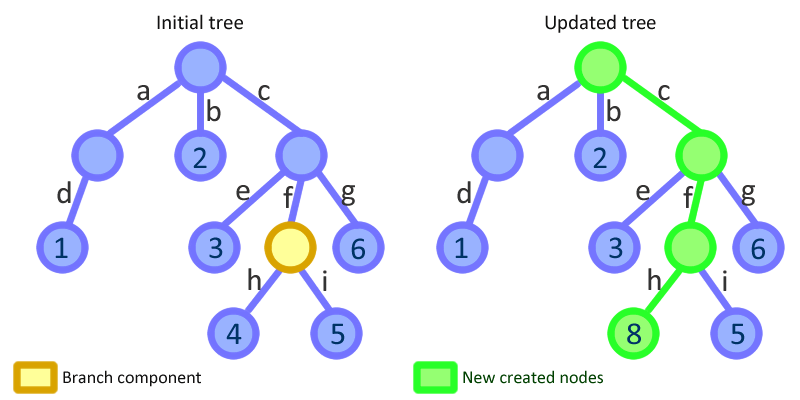
\includegraphics[scale=0.5]{obrazky/immutable_trees}
\par\end{centering}
\caption{Ukázka generování nových imutabilních objektů \cite{immutable_json} \label{fig:immutable_tree}}
\end{figure}

Číslo 4 se v ukázce změnilo na 8, ale více než polovina stromu zůstala zachována. Díky tomu že se jedná o reference, je jejich kopírování velmi rychlé. Nástroj immutable.js, který je dnes asi nejvhodnějším nástrojem pro práci s imutabilními objekty, je úzce svázan s frameworkem React. Síla a rychlost virtuálního DOM, který React používá, je založena na používání imutabilních objektů. Díky nim můžou být operace s virtuálním DOM velmi rychlé. V následujícím grafu je vidět porovnání rychlosti vykreslování webové aplikace, využívající a nevyužívající imutabilní objekty \cite{immutability_graph}. Další zvýšení rychlosti lze docílit použitím PureRenderMixinu v React, který zajistí používání imutabilních struktur i při vykreslování komponent UI \cite{react} \cite{immutablejs_learn}.

\begin{figure}[h]
\begin{centering}
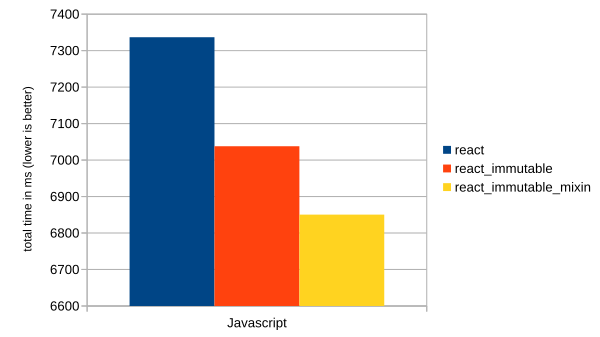
\includegraphics[scale=0.6]{obrazky/immutable}
\par\end{centering}
\caption{Graf rychlostí vykreslování aplikace v React s využitím nebo nevyužitím imutabilních objektů. \cite{immutability_graph} \label{fig:react_immutable}}
\end{figure}
\FloatBarrier 

\section{Vhodné programovací jazyky a nástroje}
Jediným jazykem, který je dnes použitelný na serveru i ve webovém prohlížeči je Javascript. Ten vznikl jako čistě prohlížečový jazyk a díky platformě node.js může nyný sloužit i jako serverový jazyk. Následující kapitola shrnuje nejpoužívanější knihovny a nástroje pro jazyk Javascript, spolu s popisem jejich využití v isomorfních webových aplikacích \cite{isomorhic_book}.

\subsection{node.js}
Není překvapením, že se použití node.js jako serverové části, stává přirozenou volbou nejen pro aplikace závislé na velkém javascriptovém frontendu. Je totiž velmi výhodné používat stejný jazyk pro obě části aplikace. Princip isomorfních aplikací je na používání jediného jazyka založen, použití node.js na straně serveru je tak prakticky jedinou volbou. Tyto aplikace jsou navrženy tak, aby dokázaly ekvivalentně fungovat v prohlížeči i na serveru. Obě části aplikace jsou tak schopny provádět některé operace, například šablony se vykreslují nejdříve na serveru a poté i prohlížeči. Framework React, často používaný pro tvorbu uživatelských rozhraní, funguje bezproblémově na obou prostředích. Serverová část aplikace funguje nejčastěji za pomocí frameworku \textit{express}, který v node.js řeší běžné věci, které programátor očekává od serverového frameworku v některém z běžně používaných jazyků \cite{glover_nodejs} \cite{tilkov_nodejs} \cite{isomorhic_book}.

\subsection{npm}
Balíčkovací systém npm (viz \hyperref[sec:node_js]{2.4}), původně vzniklý pro potřeby serverové platformy node.js, dnes nachází místo i jako systém správy závislostí pro klientskou část aplikace, kde se vždy používal například Bower nebo podobné nástroje \cite{bower}. Npm se stává standardem pro definování závislostí webových aplikací, nalezneme tam téměř všechny běžně používáné javascriptové knihovny. Proto je více než vhodný pro použití v isomorfních aplikacích \cite{npm} \cite{isomorhic_book}.

\subsection{express}
Express je serverový framework pro node.js určený k programování webového serveru v jazyce Javascript. Slouží pro vykreslování HTML, komunikaci s databází, rozhraní pro tvorbu API a další věci, které řeší běžný webový framework v některém ze známých serverových jazyků (PHP, ASP.NET, Python) \cite{express}.

Následující ukázka kódu ilustruje vykreslení HTML šablony pro stránku example.
\begin{lstlisting}[language=Javascript, caption= Ukázkové vykreslení šablony pomocí frameworku express \cite{express}]
var exampleProvider = require('../providers/ExampleProvider'), menuStructure = require('../MenuStructure');

// request handler pro /example
module.exports = function(app) { app.get('/example', function(req, res) {
       var example = exampleProvider.getExample(); 
       var templateData = {
       title: example.title, 
       heading: example.heading, 
       content: example.content, 
       menuStructure: menuStructure
    };
res.render('example', templateData); });
}
\end{lstlisting}

\subsection{Immutable.js}
\label{sec:immutable_js}
Princip imutability dat je popsán spolu s jeho hlavními výhodami v kapitole \hyperref[sec:immutability]{4.3}, imutabilní přístup je pro isomorfní aplikace naprosto zásadní, velmi totiž urychluje práci s daty. Knihovna immutable.js od společnosti Facebook je nejpoužívanějším nástrojem pro práci s imutabilními datovými strukturami \cite{immutablejs}. Byla vytvořena v roce 2014 Lee Byronem kvůli zrychlení DOM manipulací ve frameworku React. Immutable.js nabízí několik persistentních imutabilních struktur \cite{immutablejs}: 

\begin{itemize}
\item List,
\item Stack,
\item Map,
\item OrderedMap,
\item Set,
\item OrderedSet,
\item Record,
\item lazy Seq.
\end{itemize}

Tyto struktury jsou velice rychlé a efektivní, využívají nových možností moderních javascriptových prohlížečových jader jako je \textit{structural sharing}\footnote{Možnost sdílení referencí mezi datovými strukturami.} nebo hashovací datové stromy (hash map tries)\footnote{Vyhledávací datová struktura, která asociuje hašovací klíče s odpovídajícími hodnotami. Hodnota klíče je spočtena z obsahu položky pomocí takzvané hašovací funkce.}. Tyto techniky popisují vysoce optimalizované způsoby ukládání dat. Díky nim je možné minimalizovat nutnost kopírování nebo cachování datových struktur, a tím významně zrychlit manipulace s daty \cite{immutablejs} \cite{immutablejs_learn}.

\subsubsection{List}
List je immutabilní reprezentace klasického javascriptového pole, kde ale každá změna (zpravidla realizována pomocí funkce \textit{push}) vrátí vždy nový imutabilní objekt \cite{immutablejs} \cite{immutablejs_learn}.
\begin{lstlisting}[language=Javascript,caption={Ukázka práce s imutabilním objektem List v immutable.js \cite{immutablejs}}]
var list1 = Immutable.List.of(1, 2);
var list2 = list1.push(3, 4, 5);
\end{lstlisting}

\subsubsection{Stack}
Stack je datová struktura typu FILO\footnote{first in, last out}, která reprezentuje zásobník. Lze si ho představit jako pole, kde první index ukazuje na element, který může být vyjmut pomocí metody \textit{pop()}. Ostatní elementy jsou dostupné pomocí getteru přijímacího index elementu. Modifikace zásobníku, pomocí metod \textit{push()} a \textit{pop()} vrací vždy nový imutabilní zásobník \cite{immutablejs} \cite{immutablejs_learn}.
\begin{lstlisting}[language=Javascript,caption={Ukázka práce s imutabilním objektem Stack v immutable.js \cite{immutablejs}}]
var filo = new Immutable.Stack();
var twoStoreyStack = filo.push( '2nd floor', '1st floor', 'ground floor' );
twoStoreyStack.size // 3
twoStoreyStack.get(1) // "1nd floor"
twoStoreyStack.pop()
twoStoreyStack.size // 2
\end{lstlisting}

\subsubsection{Map}
Imutabilní mapa je klasickou implementací key –> value mapy využívající hashovací funkci. Chová se opět naprosto stejně jako běžná javascriptová mapa, jen každá změna (přidání nebo odebrání objektu) vrátí novou imutabilní mapu \cite{immutablejs} \cite{immutablejs_learn}.
\begin{lstlisting}[language=Javascript,caption={Ukázka práce s imutabilními mapami v immutable.js \cite{immutablejs}.}]
var Immutable = require('immutable');
var map1 = Immutable.Map({a:1, b:2, c:3});
var map2 = map1.set('b', 50); //změna imutabilního objektu, vrátí novou instanci
map1.get('b'); // 2
map2.get('b'); // 50
\end{lstlisting}

\subsubsection{OrderedMap}
OrderedMap je implementace seřazené mapy, vzhledem k imutabilitě ale změna hodnoty na některém z klíčů, nevyvolá opětovné seřazení. To je nutné zajistit ručně pomocí metod \textit{sort()} nebo \textit{sortBy()}, které také, dle očekávání, vrací novou imutabilní mapu \cite{immutablejs} \cite{immutablejs_learn}.
\begin{lstlisting}[language=Javascript,caption={Ukázka práce s imutabilními seřazenými mapami v immutable.js}]
var basket = Immutable.OrderedMap()
                      .set( 'Captain Immutable 1', 495 )
                      .set( 'The Immutable Bat Rises 1', 995 );

console.log( basket.first(), basket.last() ); // 495 995
var basket2 = basket.set( 'Captain Immutable 1', 1095 );
var basket3 = basket2.sortBy( (value, key) -> -value); 
console.log(basket3.first(), basket3.last()); // 995 1095
\end{lstlisting}

\subsubsection{Set}
Imutabilní set je pole unikátních elementů, s obvyklími obslužnými metodami. Přidávání elementů se realizuje pomocí funkce \textit{add()}. Teoreticky tato datová struktura nezajišťuje pořadí uložených elementů. Přidání nebo odebrání elementu vždy vytvoří novou instanci imutabilního setu \cite{immutablejs} \cite{immutablejs_learn}.

\begin{lstlisting}[language=Javascript,caption={Ukázka práce s imutabilním objektem Set v immutable.js \cite{immutablejs}}] 
var s1 = Immutable.Set( [2, 1] );
var s2 = Immutable.Set( [2, 3, 3] );
var s3 = Immutable.Set( [1, 1, 1] );
console.log( s1.count(), s2.count(), s3.count() ); // 2 2 1
\end{lstlisting}

\subsubsection{OrderedSet}
OrderedSet se implementace imutabilního setu s daným pořadím. Elementy jsou řazeny dle data přidání. Jeho použití je totožné s klasickém imutabilním setem, který ale nezaručuje pořadí elementů. Je proto doporučeno používat OrderedSet všude tam, kde je nutné pracovat s elementy ve správném pořadí  \cite{immutablejs} \cite{immutablejs_learn}.

\subsubsection{Record}
Record je imutabilní reprezentací javascriptové třídy s výchozími hodnotami. Je nutné ho instancovat pomocí operátoru \textit{new} jako běžnou třídu. Často slouží jako imutabilní obálka pro datové entity. Dotazování na data funguje pomocí přímého přístupu k vlastnostem objektu, pokud není vlastnost nastavena, vrátí se výchozí hodnota dle definice struktury Record \cite{immutablejs} \cite{immutablejs_learn}.
\begin{lstlisting}[language=Javascript,caption={Ukázka práce s imutabilním objektem Record v immutable.js \cite{immutablejs}}]
var Canvas = Immutable.Record( { width: 1024, height: 768 } );
var myCanvas = new Canvas();
console.log(myCanvas.toJSON()); // Object {width: 1024, height: 768}
console.log(myCanvas.width); // 1024
var myResizedCanvas = new Canvas( {width: 400} );
console.log(myCanvas.toJSON()); // Object {width: 400, height: 768}
console.log(myCanvas.width); // 400
\end{lstlisting}

\subsubsection{lazy Seq}
Knihovna immutable.js také přináší datovou strukturu lazy Seq, česky líná sekvence, která slouží jako imutabilní obálka nad libovolnou kolekcí. Seq umožňuje využívat efektivní funkcionální programování pomocí metod \textit{map} nebo \textit{filter}. Často se používá pro procházení nebo vyhledávání v datových kolekcích. Struktura je lazy, to v programátorské terminoligii znamená, že k jejímu vyhodnocení dojde až při jejím prvním použití, což je zajímavá vlastnost, která také zvyšuje výkon aplikace využívající imutabilní přístup \cite{immutablejs} \cite{immutablejs_learn}.
\begin{lstlisting}[language=Javascript, caption={Ukázka používání lazy Seq v immutable.js \cite{immutablejs_learn}}] 
var seasons = Immutable.Seq( ['spring', 'summer', 'fall', 'winter'] )
                     .filter( season -> season[0]==="s") // pouze začínající na "s"
                     .map(String.toUpperCase);
 
console.log( 'Item at index 0: ', seasons.get( 0 ) ); // SPRING
console.log( 'Item at index 1: ', seasons.get( 1 ) ); // SUMMER
console.log( 'Seasons in an array: ', seasons.toJS() );
\end{lstlisting}

\subsection{React}
\label{sec:react_isomorphic}
Knihovna React, popsaná v kapitole \hyperref[sec:react]{2.8.3} je nejpoužívanější knihovnou pro prezentační vrstvu ve světě isomorfních aplikací. Její úzké zaměření pouze na vykreslování HTML je pro její použití ideální. React také bez problému běží v prostředí node.js, je tedy možné šablony jednoduše vykreslit na serveru a ušetřit tak část práce webovému prohlížeči \cite{react} \cite{react_intro}.
 
Dále následuje popis hlavních částí a implementační detaily knihovny React ve vztahu k programování isomorfních webových aplikací \cite{isomorhic_book}.

\subsubsection{Komponenty}
Základní programovou jednotkou frameworku React je komponenta. Za komponentu lze označit libovolnou část HTML dokumentu, která označuje konkrétní část uživatelského rozhraní webové aplikace. Komponenty slouží pro vykreslování dat. Mohou se libovolně zanořovat, každá komponenta tedy obvykle obsahuje další (vlastněné) komponenty. Vzhledem k tomu, že je v React doporučováno používat syntaxe ES6, lze na každou komponentu nahlížet jako na třídu, přesněji na potomka třídy \textit{React.Component}. Každá komponenta musí implementovat metodu \textit{render()}, ve které je deklarativně definováno související uživatelské rozhraní. To je vždy tvořeno existujícími UI komponentami, které reprezentují buď jednotlivé elementy HTML, například \textit{React.DOM.div}, \textit{React.DOM.input}, nebo jakoukoli komplexnejší programátorem definovanou HTML strukturu. Při vykreslování se komponenty chovají jako funkce, které přebírání HTML vlastnosti (viz níže) a vracejí kompletní HTML kód jednotlivé části webové aplikace \cite{react} \cite{react_intro}.

\subsubsection{Virtuální DOM}
\label{sec:virtual_dom}
DOM (Document Object Model) reprezentuje celou HTML stránku jako hierarchii entit, se kterými lze programově manipulovat pomocí Javascriptu. Možnosti práce s DOM jsou velmi bohaté, lze programově vytvářet, měnit nebo mazat HTML elementy a dostupná je také možnost práce s CSS stylováním. Tyto manipulace jsou nezbytné pro fungování jednostránkových webových aplikací i obecně celé oblasti programování webových aplikací v Javascriptu. DOM jako takový ale nebyl navržen s ohledem na masivní využívání těchto manipulací. Možnost dodatečných úprav stažené webové stránky byla využívána pouze pro jednoduché změny nebo vylepšení. Až moderní javascriptové frameworky přinesly velmi dynamická uživatelská rozhraní, na které není klasický DOM připraven. Jejich obsluha vyžaduje provádět mnoho složitých DOM manipulací, které jsou, při velkém počtu HTML elementů, velmi pomalé. Vezměme si pro představu třeba nějakou známou moderní webovou aplikaci, například Facebook nebo Instagram. Tam každou vteřinu probíhají desítky, ne-li stovky takových DOM manipulací s mnoha různými elementy. Společnost Facebook, jeden z fenoménů dnešní doby, řešila problém s nízkou rychlostí DOM manipulací a navrhla řešení zvané \textit{virtuální DOM}, které je jedním ze základních princpů knihovny React, často zmiňované v této práci. Virtual DOM značí technologii tvorby abstraktního Document Object Modelu spravovaného pomocí Javascriptu uvnitř webového prohlížeče. Framework při každém vykreslování reálného DOM vytvoří také novou verzi toho virtuálního. Nad ním jsou potom realizovány změny. Při následujícím vykreslování je porovnán reálný DOM s tím virtuálním a ta část stromu, která se změnila, se změní i v prohlížeči. Tento postup je znatelně rychlejší než práce přímo s reálným prohlížečovým DOM. Při práci s virtuálním DOM existují především dva problémy, které je třeba řešit \cite{react} \cite{virtualdom}.
\begin{itemize}
\item Kdy reálný DOM překreslovat z toho virtuálního?
\item Jak překreslovat efektivně a rychle?
\end{itemize}

Reálný DOM překreslujeme pokaždé, pokud došlo ke změně dat. A to jen těch, které má zaregistrována některá z aktuálně zobrazených komponent. Pokud se změní data, která nejsou aktuálně zobrazována, je zbytečné provádět překreslení \cite{virtualdom}. Změny v datech lze kontrolovat několika způsoby. Je možné je v pravidelném intervalu procházet a při první nalezené změně vyvolat modifikaci virtuálního a posléze i reálného DOM. Alternativní byť doporučovanou možností je vyvolání změn v DOM na základě nějaké události, například doručení dat ze serveru. Na to je ale nutné myslet při implementraci těchto událostí. Rychlé a efektivní překreslování vyžaduje obecně splňení těchto podmínek \cite{react} \cite{virtualdom}.

\begin{itemize}
\item Efektivní algoritmus pro vyhledávání změn mezi reálným a virtuálním DOM.
\item Realizace zapisovacích operací v dávkách.
\item Efektivní překreslování jen nezbytného části DOM.
\end{itemize}

Všechny zníměné problémy řeší framework React a podobné knihovny, které jsou na konceptu virtuálního Document Object Modelu vystavěny \cite{react} \cite{virtualdom}. Následující diagram dobře ilustruje fungování virtuálního DOM v React.

\begin{figure}[h]
\begin{centering}
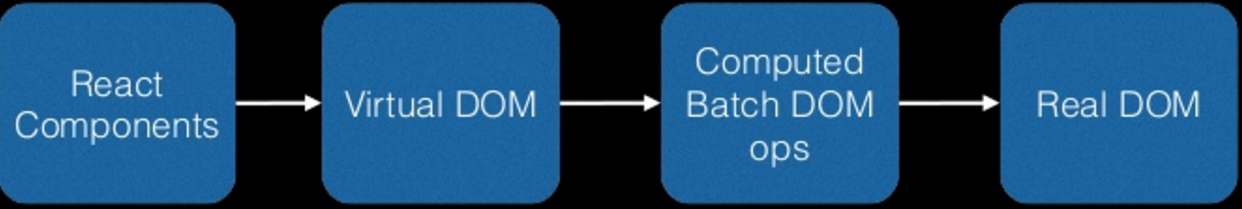
\includegraphics[scale=0.3]{obrazky/virtual_dom}
\par\end{centering}
\caption{Diagram práce virtuálního DOM v React \cite{react} \label{fig:virtual_dom}}
\end{figure}
\FloatBarrier

\subsubsection{JSX}
Jednotlivé komponenty či jejich stromy se ve frameworku React zapisují pomocí speciální syntaxe zvané JSX. Jedná se o rozšíření ECMAScriptu představené spolu s frameworkem React, které přináší novou syntaxi velmi podobnou HTML. Například zápis \textit{<div>text</div>} je frameworkem přeložen na \textit{react.default.createElement('div',null,'text')}, což je sice pochopitelnější konstrukce, ale zase se mnohem hůře čte. JSX se používá nejen pro definici HTML ale především pro řízení zobrazování jednotlivých komponent uživatelského rozhraní \cite{react} \cite{react_book}.

\begin{lstlisting}[language=Javascript,caption={Definice komponenty, která volá jiné komponenty v JSX}]
export default class CommentList extends Component {
render() {
...
  return (
  <div className='comments'>
      <ul>
          <CommentItem key={key} row={key} id={comment.id} editable={editable} comment={comments[0]} {...actions} />
           <CommentItem key={key} row={key} id={comment.id} editable={editable} comment={comments[1]} {...actions} />
            <CommentItem key={key} row={key} id={comment.id} editable={editable} comment={comments[2]} {...actions} />
      </ul>
 	);
 }
}
\end{lstlisting}

Výše uvedená ukázka kódu obsahuje vykreslovací kód komponenty \textit{CommentList} pro zobrazení komentářů v ukázkové webové aplikaci. V ukázce se kombinuje použití klasického HTML s voláním React komponent s parametry, které se nazývají \textit{props} a slouží k přenosu dat z rodičovských komponent. Za zmínku také stojí, že jsou některé HTML atributy v JSX přejmenovány. Jedná se například o atribut class, ktery se zapisuje jako className nebo for, kde se používá htmlFor. Přejmenování bylo nutné, aby nevnikaly kolize s existujícími klíčovými slovy \textit{class} a \textit{for}. Často se stává, že na to vývojář zapomene, proto to framework React dokáže rozpoznat a napoví kde je atribut nesprávně pojmenován \cite{react} \cite{react_book}.

\subsubsection{Props}
\label{sec:react_props}
Framework React rozlišuje data komponent na dva typy. Prvním z nich je stav (state), který tvoří aktuální stav dané komponenty a jen komponenta sama ho může změnit. Druhý typem jsou vlastnosti (properties, zkráceně props), které reprezentují podmnožinu dat webové aplikace a komponenta sama je nemůže nijak měnit. Tyto vlastnosti jsou neměnné a musí být komponentě explicitně předány při jejím zobrazování \cite{react_components} \cite{react_thinking}. Výše uvedená ukázka kódu používá komponentu \textit{CommentItem}, které předává props obsahující: komentář samotný (\textit{comment}), číslo řádku (\textit{row}) a přepínač editace (\textit{editable}). Následující ukázka demonstruje tuto komponentu, která se stará pouze o zobrazení předaných dat (komentářů).

\begin{lstlisting}[language=Javascript,caption={Definice komponenty CommentItem, která zobrazuje komentář}]
export default class CommnetItem extends Component{
render() {
  return(
      <div className='commentItem'>
          <p className='rowNumber'>{row+1}.</p>
          <p className='title' onClick={::this.handleClick}>{comment.text}</p>
          <p className='created'>{moment(modified).fromNow()}</p>
          <p className='outcome'>{comment.author}</p>
    </div>
  );
}
}
\end{lstlisting}

Předávat komponentám lze samozřejmě i funkce či objekty. Props fungují pouze jednosměrně směrem zhora dolů. Komponenta CommentItem nemůže nic předat rodičovské komponentě CommentList. Může však dostat od rodičovské komponenty funkci ve formě callbacku a ten zavolat. Tento jednosměrný postup velmi redukuje komplexnost webových aplikací a tím zjednodušuje správu dat v aplikaci \cite{react} \cite{react_thinking}.

Každá změna props nebo state vždy vyvolá znovuvykreslení komponenty prostřednictvým zavolání funkce \textit{render()} na té komponentě, která zaregistrovala změnu dat. Ta většinou vyvolá překreslení dalších podřízených komponent \cite{react} \cite{react_components}.

\subsubsection{States}
Celá isomorfní webová aplikace nebo všeobecně aplikace bohatě využívající Javascript jsou hluboce založeny na stavech. Nejdříve je nutné si definovat, co je vlastně stav webové aplikace. Zjednoduše řečeno je to vlastně úvodní podoba stránky společně se všemi změnami do okamžiku, kdy tento stav posuzujeme. Zahrnuje DOM elementy a jejich obsah, pořadí, atributy, ale i javascriptové proměnné apod. Způsobů jaké se dnes používají pro reprezentaci stavu webové aplikace je mnoho \cite{zakas_js} \cite{skriptovaci_jazyky}:

\begin{itemize}
\item přidáváním CSS tříd,
\item využití data-* HTML atributů,
\item použití globálních datových struktur Javascriptu ( window.data nebo \$("\#elem").data()).
\end{itemize}

V důsledku těchto postupů jsou data často nepředvídatelně poschovávána na různých místech aplikace. To přináší problémy při implementaci složitějších webových aplikací. Komponenty frameworku React pracují se svým vlastním vnitřním stavem, jehož ukládání je plně v režii frameworku. Tento stav určuje aktuální podobu dané komponenty, vždy dojde-li k jeho změně, zavolá komponenta automaticky metodu \textit{render()} a překlesí se. Změna stavu je většinou spojena například s kliknutím na tlačítko nebo se změnou souvisejícího formulářového prvku. Původní koncept frameworku React počítal s tím, že pouze komponenta sama může provádět změny svého stavu. Striktně lokální povaha tohoto stavu ale komplikuje možnosti ovládání dané komponenty, proto je dnes doporučované předávat komponentě celý její stav zvenčí pomocí parametru. Veškerá data, která komponenta potřebuje, předáváme jako její \textit{props} pomocí nadřazené komponenty. Hovoříme potom o takzvaných \uv{stateless (bezstavových) komponentách}. Všechny lokální stavy všech komponent by měly být uloženy na jednom místě. Tím místem je podle principu \uv{jediného zdroje pravdy} (single source of truth), úložiště \textit{store} z architektury Flux (viz. \hyperref[sec:flux]{4.4.6}) \cite{react} \cite{react_book}  \cite{flux} \cite{react_thinking}.

Store obsahuje všechna data aplikace a ostatní komponenty na tato data nahlíží a reagují na ně. Když se data změní, komponenty se překreslí. Žádná komponenta nikdy nezjišťuje stav jiné komponenty, vždy se dívá pouze do store. Data vyjadřují aktuální stav aplikace a stejná data musí vždy aplikaci uvést do stejného stavu. Tomuto principu se říká \uv{předvídatelný stav} (predictable state). Z takového přístupu plyne mnoho výhod. Například ladění je velmi snadné, protože všechny změny prochází jediným místem, do kterého můžeme nahlédnout. Také můžeme jednoduše implementovat funkci undo – vracení akcí zpět \cite{react_book} \cite{flux} \cite{react_thinking}.

\subsubsection{Vykreslování HTML}
Webová aplikace využívající React je vždy celá překreslena při každé změně stavu. Vývojáři tohoto frameworku zastávájí názor, že je jazyk Javascript již dostatečně výkonný, aby bylo rychlé překreslování možné. Tím je odstraněna potřeba data někde předem výpočítávat a dočasně ukládat. Veškeré výpočty by měli být prováděny až v metodě \textit{render()} každé React komponenty, aby se předešlo problémům s konzistencí dat. Vykreslování HTML probíhá pomocí volání zmíněné metody \textit{render()} od kořenové aplikační komponenty (často zvané Root nebo WebApplication) rekurzivně přes celý strom komponent. Překreslení některého z podstromů je možné pro zlepšení výkonu omezit implementováním metody \textit{shouldComponentUpdate()}, která provede porovnání aktuálního a nového stavu komponenty a vrátí pravdivostní hodnotu, zda je nutné daný podstrom překreslit nebo ne \cite{react} \cite{react_components} \cite{react_book}.

\subsubsection{Delegování událostí}
Další důležitou vlastností React je možnost delegování událostí, které zefektivňuje práci s DOM a vylepšuje práci s pamětí. Ke každé komponentě je možné přiřadit nějakou obsluhu událostí, ve skutečnosti však existuje jeden jediný posluchač, připojený na nejvyšší úrovni Document Object Modelu, jež obaluje veškeré události prohlížeče a předáva je do virtuálního DOM. To umožňuje předat obsluhu události správné komponentě aniž by docházelo ke ztrátě výkonu. Správa připojených posluchačů probíhá na interní bázi frameworku, není tedy nutné pracovat s reálným DOM. Automatická správa posluchačů je u moderního webového frameworku nezbytností \cite{react} \cite{react_components}. Podle Zakas je obrovský počet, často již nepoužívaných posluchačů navěšených na DOM elementy, jedním z hlavních zdrojů problémů s výkonem a paměťovou náročností moderních javascriptových webových aplikací \cite{zakas_js}.

\subsubsection{React router}
Velmi podstatnou částí každé webové aplikace je router, který zpracovává HTTP požadavky a podle URL a vstupních dat iniciuje příslušné části aplikace. U jednostránkových aplikací, kam isomorfní aplikace spadají, není možné použít klasický serverový MVC přístup, protože routování probíhá uvnitř webového prohlížeče. Je nutné použít nějaký router pro Javascript. Knihovna React nabízí nástroj \textit{React-router}, který řídí tok dat v aplikaci, mění aktuální URL nebo zajištuje správné fungování historie i tlačítka zpět. Router také řeší zpracování a předávání parametrů obslužným metodám. Jednotlivé definice vstupních částí aplikace spolu s připojenými React komponentami se nazývají routovací pravidla a jsou zapisována pomocí syntaxe JSX \cite{react} \cite{react_router}.

\begin{lstlisting}[language=Javascript,caption={Ukázka definice routování pomocí React-router \cite{react_router}}]
   <Router history = {browserHistory}>
      <Route path = "/" component = {App}>
         <IndexRoute component = {Home} />
         <Route path = "home" component = {Home} /> // na /home iniciuj komponentu Home
         <Route path = "about" component = {About} />
         <Route path = "contact" component = {Contact} />
      </Route>
   </Router>
\end{lstlisting}

Při použití isomorfního přístupu je většinou nutné používat jeden router na straně serveru a druhý na straně webového prohlížeče. Moderní isomorfní devstacky ale dokážou propagovat jednou definovaná routovací pravidla do obou routerů \cite{react_book} \cite{react_router}.

\subsection{Flux}
\label{sec:flux}
Společnost Facebook také navrhla architekturu správy dat známou jako Flux, která řeší mnohé problémy běžných MVC frameworků se správou dat. Jedná se o návrhový vzor, který se aplikuje při návrhu jednosměrného toku dat v aplikaci. Vychází z předpokladu, že výsledné UI je reprezentovatelné pomocí dat, které do něj tečou z úložišť (Store). Interakce uživatelů jsou reprezentovány pomocí akcí (Actions). Akce zpracovává dispečer (Dispatcher), který následně notifikuje o změnách jednotlivá úložiště, ty změnu provedou a reflektují ji do UI komponent které je poslouchají \cite{react_book} \cite{flux}.

\vspace{3mm}
\noindent Architektura flux má několik základních pravidel \cite{react_book} \cite{flux}.

\begin{itemize}
\item Všechna data v úložištích mohou být měněny pouze skrz akce.
\item Všechny akce vstupují do úložiště skrze jediný bod vstupu 
\item Není možné provést novou akci dokud ta aktuální neskončí. To také znamená, že všechny úložiště jsou zaktualizovány najednou, a vždy nechají aplikaci v konzistentním stavu (princip transakce).
\item Data uvnitř úložišť jsou přístupná z vnějšku pouze skrz read-only veřejné API.
\end{itemize}

Důsledkem jejich dodržování je to, že v jakýkoliv okamžik je velice jednoduché si udělat představu o tom, co se uvnitř úložišť děje \cite{react_book}. Následující obrázek dobře ilustruje fungování celé architektury.

\begin{figure}[h]
\begin{centering}
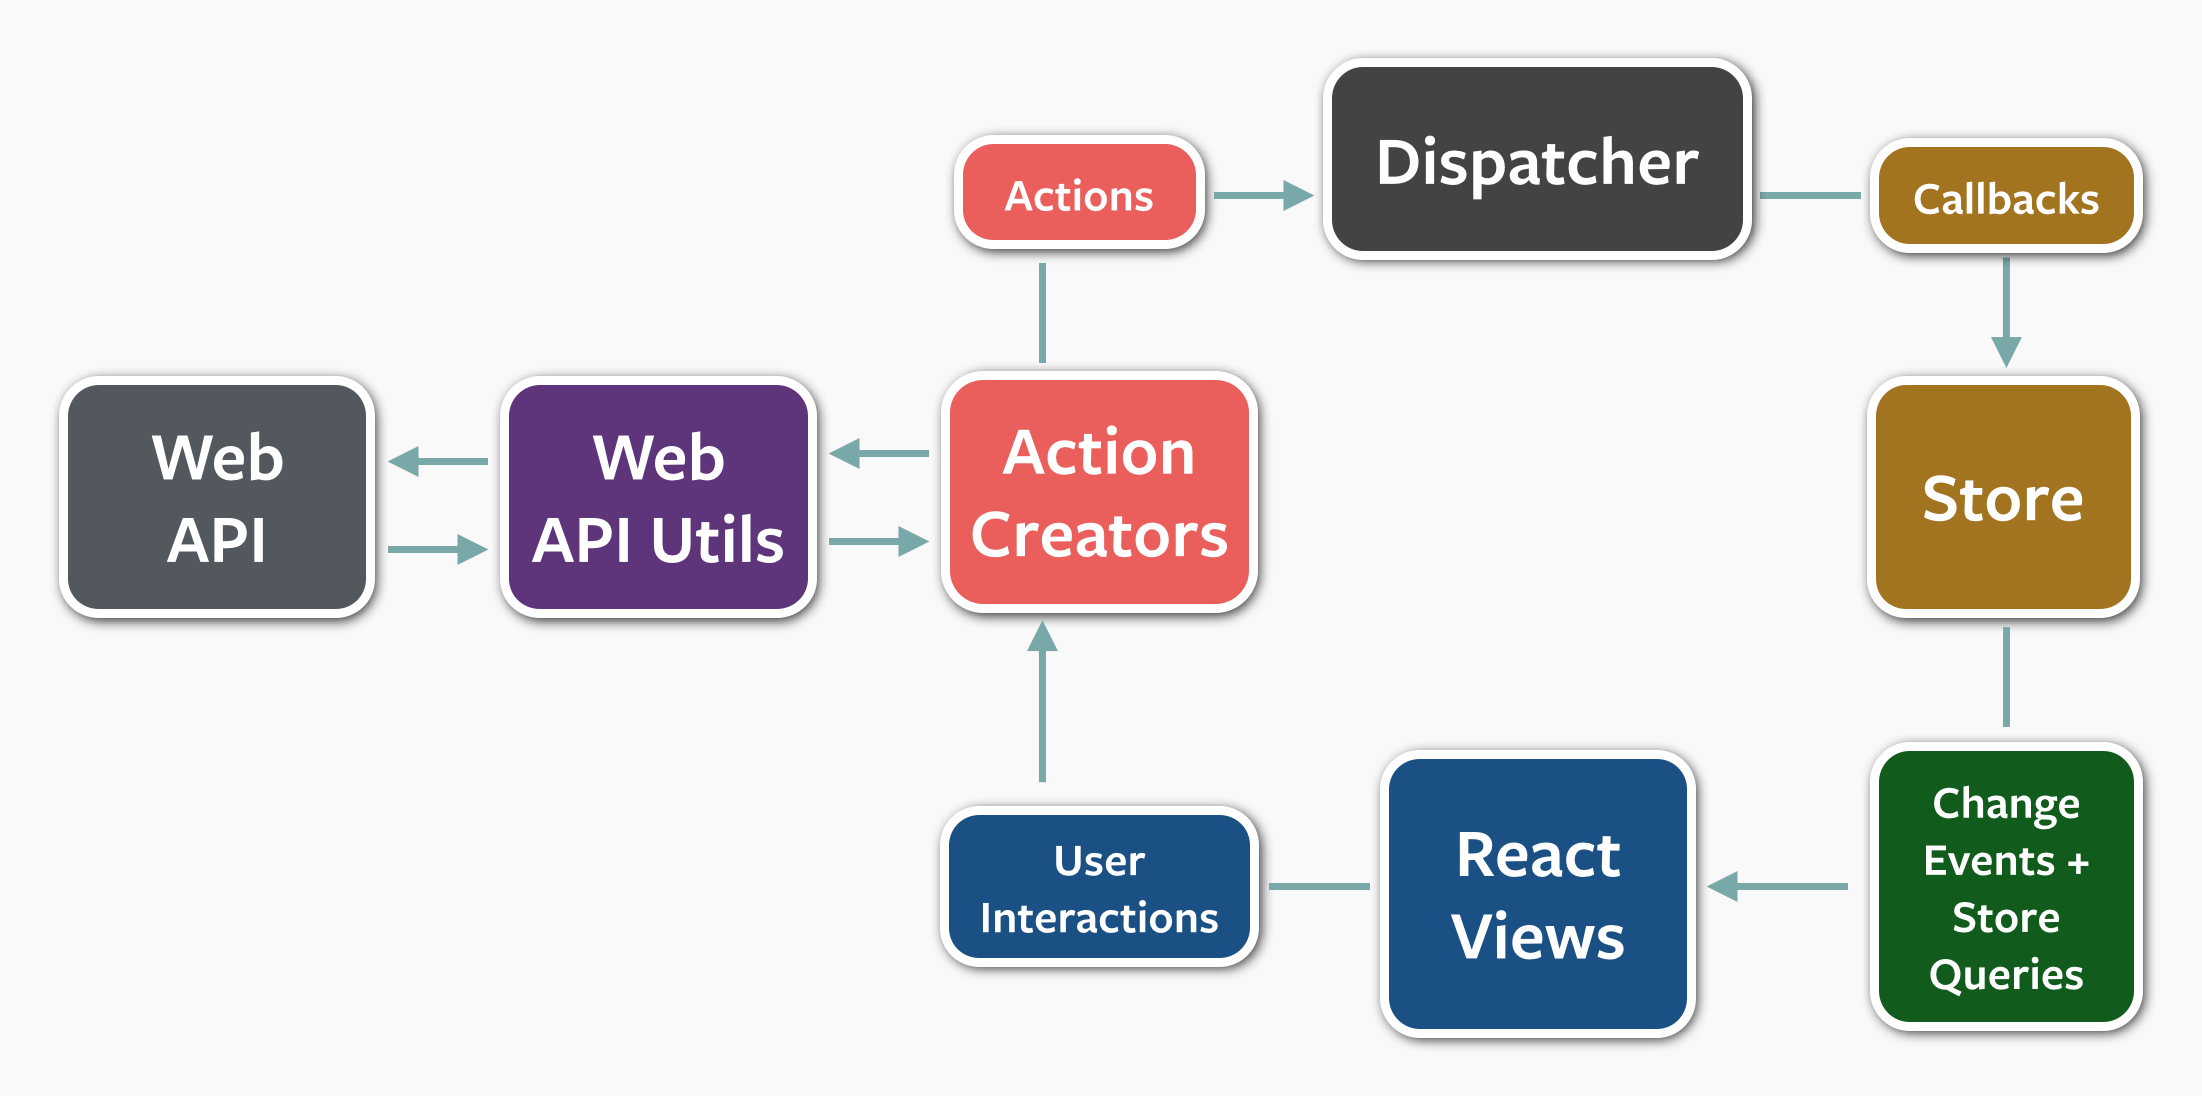
\includegraphics[scale=0.3]{obrazky/flux_architecture}
\par\end{centering}
\caption{Diagram architektury Flux \cite{flux} \label{fig:flug_architecture}}
\end{figure}
\FloatBarrier

I když Flux přináší mnoho výhod a řeší některé aktuální problémy javascriptových aplikací, má také mnoho nevýhod. Především je to pomalá křivka učení, nové implementační koncepty a složitý kód. Flux jako takový je ale pouze návrhovým vzorem, který nelze stáhnout a používat. Je nutné použít některou z jeho implementací. Mezi neznámější z nich patří \textit{Redux}, \textit{Delorean}, \textit{Lux}, \textit{Reflux} nebo \textit{OmniscientJS} \cite{flux_comparison}. První jmenovaný je v současné době doporučovaný a používá ho i ukázková aplikace v této práci. Redux je predikovatelný stavový kontejner pro javascriptové aplikace. Pomáhá psát konzistentní, dobře testovatelné aplikace, které můžou běžet na všech dostupných javascriptových platformách. Vývojářům také přináší nové možnosti jako je živá editace kódu nebo time-traveling debugger\footnote{Debugování, při kterém lze přepínat mezi předchozími aplikačními stavy a tím se fakticky \uv{vracet v čase}.}. Redux pracuje dle principu Flux, ale dispatcher nahrazuje takzvaným \textit{reducerem}. Jedná se o obyčejnou funkci, která je vložena do úložiště, aby bezpečně modifikovala data dle proběhlých akcí. V momentě doručení akce do úložiště, je zavolán reducer kterému je předán současný stav aplikace a provedené akce. Uvnitř reduceru je kód, který podle identifikace akce provede požadovanou změnu dat a vrátí jejich novou podobu – nový aplikační stav \cite{flux} \cite{redux}.

\subsection{Task runnery}
\label{sec:task_runners}
Svět programování webových aplikací v Javascriptu se neobejde bez používání mnoha knihoven. Je tedy zapotřebí někdo, kdo pomůže zautomatizovat proces vývoje například tím, že bude kontrolovat syntaxi CSS a Javascript souborů, kompilovat soubory z CSS preprocesorů (LESS, SASS, Stylus) do CSS, překompilovávat CoffeeScript do čistého Javascrptu, spojovat soubory, minifikovat, nasazovat do různých prostředí nebo generovat dokumentaci podle JSDoc. Tento proces se také nazývá buildování webové aplikace. Pro tento účel se používají knihovny zvané task runnery, většinou implementovány v Javascriptu pomocí node.js. Pro jejich docenění je nejdříve potřeba pojmenovat zásadní problém, kterému vývojáři webových aplikací čelí. Webové aplikace jsou distribuovány pomocí pomalého a nespolehlivého protokolu HTTP do vzdáleného prohlížeče. Tam se musí celá webové stránka zpracovat, spustit a něco vykonat. Výsledná velikost webové aplikace je tedy značně limitována, protože příliš dlouhé načítání je dnes zásadní problém. Aby vše fungovalo svižně, je třeba co nejvíce omezit množství nezbytných HTTP dotazů a co nejvíce minimalizovat jejich velikost. Jinými slovy je nutné pečlivě zvážit, co a kdy posílat do webového prohlížeče, v jakém pořadí a po jakých částech. Pro většinu webových aplikací stačí celou aplikaci spojit do jednoho souboru, pojmenovaného například \textit{app.js}. Tento způsob je často využíván v task runnerech Grunt a Gulp. Ovšem tento soubor může mít časem značnou velikost, proto je také možné sestavit (build) webovou aplikaci jako více ucelených částí dle jejich účelu, a ty poté dodávat do jednotlivých webových stránek. To doporučuje jiný task runner \textit{Webpack} \cite{webpack}. Tyto tři dnes nejpoužívanější task runnery, jsou popsány na následujících řádcích. Existuje více takových nástrojů, tři zmíněné jsou však současným mainstreamem pro vývoj v Javascriptu \cite{task_runners} \cite{zdrojak_gulp}.

\vspace{0,3cm}
\noindent Všechny tři zmiňované nástroje mají několik společných vlastností \cite{zdrojak_gulp}.
\begin{itemize}
\item Jsou napsány v Javasciptu – pro svůj běh vyžadují nodejs.
\item Ovládají se prostřednictvím příkazové řádky.
\item Mají velmi aktivní komunitu 
\item Každý trochu jiným způsobem řeší identickou oblast vývojářského života.
\item Opensource licence MIT
\end{itemize}

\subsubsection{Grunt}
Grunt.js byl jedním z prvních task runnerů a rychle si ho oblíbila celá Javascriptová komunita. Jeho autorem je Ben Alman a vznikl v roce 2012 \cite{grunt_intro}. Tento nástroj slouží pro automatizaci opakovaných úloh při vývoji javacriptové aplikace. Grunt upřednostňuje psaní konfigurace před psaním kódu \cite{grunt}. 

\pagebreak
\noindent Krátká ukázka toho, jak vypadá soubor Gruntfile.js \cite{grunt} \cite{zdrojak_gulp}:
\begin{lstlisting}[language=Javascript,caption={Ukázka syntaxe souboru Gruntfile.js}]
module.exports = function(grunt) {
  grunt.initConfig({
    uglify: {
    something: {
     files: {
       'dest/output.min.js': ['src/input1.js', 'src/input2.js']
     }
    }
   }
  });
  // načteme externí modul
  grunt.loadNpmTasks('grunt-contrib-uglify');
  // přidáme úlohu
 grunt.registerTask('stable-build', ['...', '...']);
};
\end{lstlisting}
\noindent Některé nevýhody task runneru Grunt \cite{zdrojak_gulp}:
\begin{itemize}
\item Konfigurace místo psaní Javascript kódu, konfigurační soubory Gruntfile jsou zpravidla delší.
\item Velké množství parametrů pro konfiguraci jednotlivých pluginů.
\item Je pomalejší při zpracování většího počtu souboru (příliš mnoho I/O operací).
\item Konkurenční zpracování úloh se řeší složitěji nebo prostřednictvím pluginu.
\end{itemize}

\subsubsection{Gulp}
Grunt klade důraz na konfigurovatelnost, takže je vhodnější pro uživatele, kteří chtějí spíše konfigurovat, než psát vlastní kód. Tím vzniká u větších projektů často obrovský a nepřehledný konfigurační soubor Gruntfile. Nástroj Gulp jde cestou psaní vlastního kódu, díky čemu je konfigurace kratší a srozumitelnější. Gulp vznikal v polovině roku 2013 pod hlavičkou společnosti Fractal. Jeho autorem je Eric Schoffstall. Jeho cílem bylo vše zjednodušit a zrychlit. Gulp masivně využívá node.js streamy, díky čemuž je většinou rychlejší než konkureční nástroj Grunt. Data se mezi jednotlivými úlohami předávají prostřednictvím pipeline\footnote{Zřetězené zpracovávání dat ve kterém výstup první části je vstupem té druhé a tak dále.}. Redukuje se tím počet I/O diskových operací a úlohy se dají snadno řetězit \cite{gulp} \cite{gulp_web} \cite{zdrojak_gulp}.

\pagebreak
\vspace{0.3cm}
\noindent Krátký příklad, jak může vypadat Gulpfile.js \cite{zdrojak_gulp}:
\begin{lstlisting}[language=Javascript,caption={Ukázka syntaxe souboru Gulpfile.js}]
var gulp = require('gulp'),
var uglify = require('gulp-uglify');
gulp.task('compress', function() {
  gulp.src(['lib/*.js'])
    .pipe(uglify())
    .pipe(gulp.dest('dist'))
});
gulp.task('default', function() {
  gulp.run('compress');
});
\end{lstlisting}

Zde je dobře viditelná základní myšlenka task runneru Gulp: Stručný a přehledný kód je lepší než složitá konfigurace \cite{gulp} \cite{zdrojak_gulp}.

\vspace{0,3cm}
\noindent Některé nevýhody task runneru Gulp \cite{zdrojak_gulp}.
\begin{itemize}
\item Masivní používání streamů může být pro začátečníka matoucí. 
\item Složitý postup pří řešení lineární závislostí jednotlivých úloh.
\item Obvykle minimální možnosti konfigurace pluginu.
\item Menší množství pluginů.
\end{itemize}

\subsubsection{Webpack}
\label{sec:webpack}
Nový nástroj pro automatizaci vývoje, přinášející opět nové koncepty se jmenuje Webpack. Ten sice vyšel už v roce 2012, ale začíná se masivně používat až v posledních zhruba dvou letech. Jeho autorem je Tobias Koppers. Webpack se oficiálně označuje jako \textit{module bundler}, není tedy typickým task runnerem, i když dokáže Gulp nebo Grunt často plně nahradit. Správu závislostí ale řeší zcela jiným způsobem, jediné co vývojář webové aplikace musí udělat, je vždy explicitně uvádět závislosti. Webpack pak potom celou aplikace projde a vytvoří kompletní graf závislostí. Na základě něj potom sestaví jeden nebo více výstupních souborů, zvaných \textit{bundles} \cite{webpack} \cite{webpack_book}.

\begin{figure}[h]
\begin{centering}
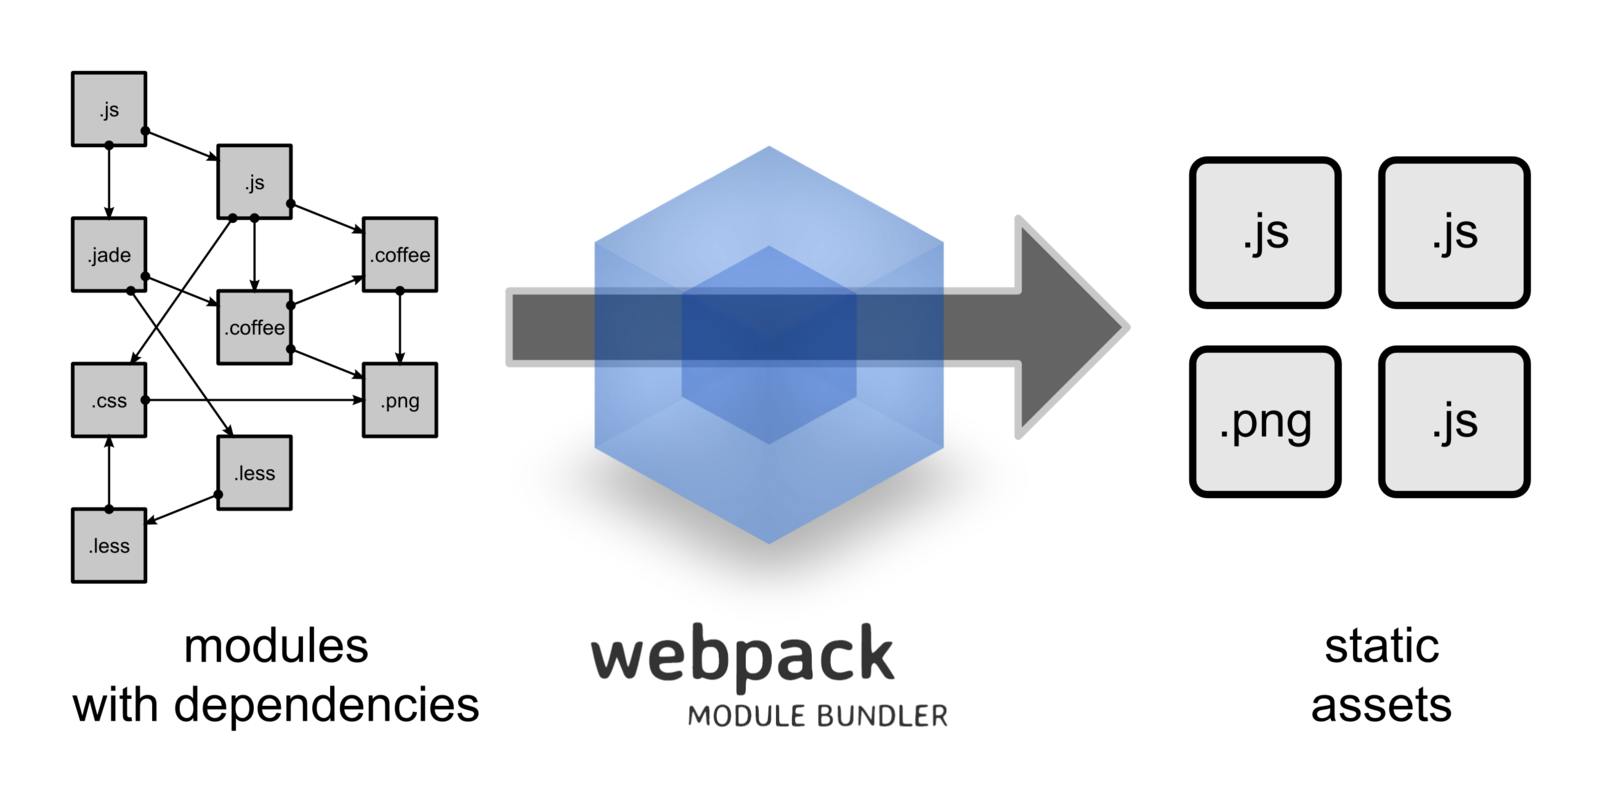
\includegraphics[scale=0.7]{obrazky/webpack}
\par\end{centering}
\caption{Diagram ilustrující způsob fungování module bundleru Webpack \cite{webpack_book}. \label{fig:webpack}}
\end{figure}
\FloatBarrier

Je nutné nakonfigurovat vstupní bod aplikace, ze kterého je zahájeno prohledávání a definovat jednotlivé loadery. Loader v kontextu Webpacku znamená program, který umí číst a zpracovávat nějaký formát. Myšlenka webpacku totiž spočívá v tom, že je možné explicitně uvádět (importovat) Javascript, CSS, obrázky, fonty a vlastně úplně cokoliv co daná stránka nebo komponenta potřebuje. Stačí použít správný loader pro všechny formáty. Výstup pak bude 100\% optimální. Každá část aplikace dostane jen tolik zdrojů, kolik skutečně potřebuje a nic zbytečně navíc. Mezi často používané loadery patří například SASS-loader nebo Babel-loader. Webpack také řeší spuštění a správu vlastního vývojového webového serveru. Tento server si hlídá všechny podmíněné soubory, tedy soubory, které jsou zdrojové pro výsledný bundle a pokud se některý z nich změní, hned vygeneruje nový bundle \cite{webpack} \cite{webpack_book}.

Jednou z nejzajímavějších vlastností Webpacku je Hot Module Replacement, česky výměna modulů za běhu. Díky tomu je možné vyměňovat části aplikace bez nutnosti jejího restartu. Webpack automaticky do každého vygenerovaného bundle přidá krátký kód, který běží uvnitř spuštěné aplikace. Když se něco v aplikaci změní (tedy vznikne nový bundle), přidáný kód nahlásí změnu daného modulu webpacku. Ten se potom pokusí nahradit pouze změněný modul, pokud to není možné, nahradí rodičovský modul. To se opakuje dokud není nahrazení provedeno nebo HMR dosáhnul vstupního bodu aplikace a nahrazení za běhu tak není možné provést. Potom dojde k chybě a je nutné provést restart celé aplikace. Webpack je velký a mocný nástroj, který je zároveň i extrémně modulární díky obrovskému množství loaderů a pluginů. Není však úplně snadné ho nastavit \cite{webpack} \cite{webpack_book}. Následuje ukázka jeho základní konfigurace, reálná konfigurace bývá násobně složitější. Hlavní částí je definice \textit{loaderů}, které zpracovávají jednotlivé soubory. 

\pagebreak
\begin{lstlisting}[language=Javascript,caption={Ukázka konfigurace module bundleru Webpack}]
module.exports = {
  entry: './main.js', // definice vstupního bodu aplikace
  output: {
    filename: 'bundle.js' // výstupní soubory
  },
  module: { 
    loaders: [ // jednotlivé loadery pro dané jazyky
      { test: /\.coffee$/, loader: 'coffee-loader' }, // loader pro coffeescript
      {
        test: /\.js$/,
        loader: 'babel-loader', // loader pro Babel
        query: { presets: ['es2015', 'react']} // Babel presety
      }
    ]
  }
};
\end{lstlisting}

\section{Ukládání dat}
Jako datová úložiště používají moderní javascriptové webové aplikace většinou NoSQL databáze. Tyto databáze nemají definovaná schémata, strukturu dat lze vynutit pouze validačními funkcemi. Ukládání dat se většinou realizuje pomocí formátu JSON, hovoříme potom o \textit{JSON dokumentu}. JSON je textový formát vycházející z podmnožiny syntaxe objektových literálů Javascriptu, je tvořen dvojicemi klíč-hodnota, kde hodnotou může být další taková dvojice, proto je libovolně strukturovatelný \cite{json}. O dokumentu hovoříme tehdy, obsahuje-li datový model  většinu souvisejících dat přímo v sobě, ne ve formě odkazů na další entity, analogie s běžným papírovým dokumentem. Tyto dokumenty často kopírují datové entity v Javascriptu \cite{ja}. Mezi často používané NoSQL databáze například MongoDB, v posledních letech je také populární realtime databáze RethinkDB, která je díky své rychlosti a dobré škálovatelnosti velmi vhodná pro isomorfní webové aplikace \cite{rethinkdb}. Je také použita v ukázkové aplikaci, popsané v praktické části práce.

\section{Vybrané devstacky}
\label{sec:devstacks}
Každé vývojové prostředí javascriptového projektu se obecně skládá z množiny spolupracujících knihoven, běžících pomocí node.js, jejichž vzájemnou interakci může být složité nakonfigurovat. Připravený soubor knihoven nebo frameworků, spolu s nástroji pro usnadnění práce vývojáře, se nazývá \textit{devstack}. Ten řeší komunikaci mezi jednotlivými částmi aplikace, sestavování (build) aplikace, řízení vývojového webového serveru nebo spouštění testů. Devstacky pro isomorfní webové aplikace řeší především níže uvedené požadavky. V závorce jsou vždy nejznámější používané javascriptové knihovny, které tyto oblasti pomáhají řešit \cite{isomorphic_pimentel}.

\begin{itemize}
\item Zpracovávání HTTP requestů (Superagent, Axios).
\item Routování URL (Director, react-router).
\item Vykreslování HTML (React, Handlebars).
\item Podporu modularizace (FormatJS, Browserify, Webpack).
\item Nástroje pro sestavení aplikace, task runnery (Webpack, Grunt, gulp.js).
\item JS transpilery (Babel, CoffeeScript, Purescript).
\item CSS procesory (Sass, Less).
\item Polyfilly pro podporu starších prohlížečů.
\item Minifikační, obfuskační nástroje (uglify.js, JSMin, CSSMin).
\item Knihovny pro isomorfní přístup (babelify, browserify, isomorphic-tools).
\end{itemize}

Následující kapitola se zabývá představením pěti vybraných devstacků vhodných pro vývoj isomorfních webových aplikací v jazyce Javascript.

\subsection{Este.js}
Prvním vybraným devstackem je Este.js, které vyšlo v roce 2013. Jedná se o isomorfní devstack od českého vývojáře Daniela Steigerwalda. Este.js samo sebe popisuje jako: \uv{nejbohatší starter kit\footnote{Připravené vývojové prostředí s příklady vhodnými pro seznámení se s danou technologií.} pro vývoj isomorfních funkcionálních webových aplikací} a jeho motto je: \textit{zapomeňte na frameworky, učte se návrhové vzory}. Což je do značné míry příznačné, protože knihoven existuje mnoho, zatímco návrhových vzorů méně a jejich znalost je pro vývoj webových aplikací důležitější. Este používá Facebook architekturu uživatelského rozhraní, Redux pro správu aplikačních stavů a programuje se v moderním ES6 Javascriptu. Zajímavostí může být použití statického type checkeru, který pomáhá objevovat nečekané chyby pomocí vyhodnocování datových typů v Javascriptu. Este neřeší otázku výběru vhodné databáze, autor však doporučuje použití Firebase. Devstack je dostupný na serveru GitHub \cite{este} \cite{isomorphic_pimentel}.

\vspace{0,3cm}
\noindent \textbf{Použité technologie}:
\begin{itemize}
\item \textbf{React} – komponenty UI.
\item \textbf{Redux} – implementace Flux architektury pro správu dat.
\item \textbf{ExpressJS} – serverová část.
\item \textbf{BabelJS} – transpiler ES6 Javascriptu.
\item \textbf{FlowType} – static type checker.
\item \textbf{react-router} – routování uživatelských požadavků.
\item \textbf{Jest} – unit testování.
\end{itemize}

\begin{table}[h]
\centering
	\caption{Výhody a nevýhody isomorfního devstacku Este.js \cite{isomorphic_pimentel}}
	\begin{tabular}{ |C{5cm}|C{5cm}| }
	\hline
	Výhody & Nevýhody \\ \hline
	UI architektura Facebooku & Málo kvalitní dokumentace a příkladů \\ \hline
	Kompletní podpora server-side renderingu & Časté změny implementace\\ \hline
	Používání ES6 Javascriptu & Známější jen v českém prostředí.\\ \hline
	Imutabilní globální stav aplikace & Větší křivka učení\\ \hline
	Skvělý výkon & \\ \hline
    \end{tabular}
	\label{tab:proscons_este}
\end{table}
\FloatBarrier

\subsection{IMA.js}
IMA.js je další český devstack, od společnosti Seznam, která ho nejdříve vytvořila pro interní účely, aby ho potom uvolnila jako open source na serveru GitHub. Je také postaven na zobrazovací vrstvě v React a backendu nad node.js pomocí Expressu. V současnosti ho používá například herní portál hry.cz. IMA.js neřeší otázku persistence dat, výběr databáze a implementace komunikace s ní je tedy čistě na programátorovi \cite{ima}.

\pagebreak
\vspace{3mm}
\noindent \textbf{Použité technologie}:
\begin{itemize}
\item \textbf{React} – komponenty UI.
\item \textbf{ExpressJS} – serverová část.
\item \textbf{BabelJS} – transpiler ES6 Javascriptu.
\item \textbf{Superagent} – framework pro komunikaci s API.
\item \textbf{Jasmine} – unit testování.
\item \textbf{Winston} – logování.
\end{itemize}

\begin{table}[h]
\centering
	\caption{Výhody a nevýhody isomorfního devstacku IMA.js \cite{ima}}
	\begin{tabular}{ |C{5cm}|C{5cm}| }
	\hline
	Výhody & Nevýhody \\ \hline
	Kvalitní dokumentace & Téměř nulová komunita \\ \hline
	Kompletní podpora server-side renderingu & Složitější konfigurace \\ \hline
	Využití nejmodernějších knihoven & Vytvořeno pro interní využití jedné firmy \\ \hline
	Jednoduché testování & \\ \hline
    \end{tabular}
	\label{tab:proscons_ima}
\end{table}
\FloatBarrier

\subsection{Meteor}
Jedním z nejpopulárnějších devstakců je také Metero, ten byl představen v prosinci roku 2011 týmem vývojářů z technologického akcelerátoru Y-Combinator. Jedná se o sadu nástrojů, které vývojářům pomáhají s vývojem webových nebo mobilních aplikací. Meteor řeší frontend, backend, balíčkování i nasazování, jeho filozofie zní \textit{Javascript everythere}. Společnost, která vznikla pro zastřešení jeho dalšího vývoje, dostala v roce 2012 investici 11,2 milionu dolarů od několika amerických investorských skupin. Je to první javascriptový nástroj, který získal investici v podobné výši. Díky ní byl zahájen bouřlivý vývoj Meteoru, který vyústil v implementaci vlastního testovacího, šablonovacího i balíčkovacího systému. Právě používání vlastních řešení a snaha o přílišnou komplexnost jsou v Meteoru často terčem kritiky. Synchronizace mezi klientem a serverem řeší Meteor zcela automaticky pomocí protokolu Websocket. Další zajímavostí je provádění databázových operací na klientu i na serveru. Meteor obsahuje \textit{minimongo}, což je implementace databáze MongoDB v Javascriptu pro použití v prohlížeči. Data se tak ukládají ihned lokálně a poté jsou asynchronně replikována do hlavní MongoDB databáze \cite{isomorphic_pimentel} \cite{meteor} \cite{meteor_web}.

\vspace{0,3cm}
\noindent\textbf{Použité technologie}:
\begin{itemize}
\item \textbf{Blaze} – reaktivní UI komponenty.
\item \textbf{DDP} – real-time komunikační protokol pro Websocket.
\item \textbf{Minimongo} – jednoduchá databáze pro webový prohlížeč replikovaná do hlavní databáze.
\item \textbf{MongoDB} – jediná kompatibilní hlavní databáze.
\item \textbf{Velocity} – testovací framework.
\end{itemize}

\begin{table}[h]
\centering
	\caption{Výhody a nevýhody isomorfního devstacku Meteor \cite{isomorphic_pimentel}}
	\begin{tabular}{ |C{5cm}|C{5cm}| }
	\hline
	Výhody & Nevýhody \\ \hline
	Velmi jednoduché na použití, mnoho kvalitní dokumentace a příkladů. & Funguje pouze s MongoDB (na Redis implementaci se pracuje). \\ \hline
   Připravený autentizační nástroj & Pouze částečná podpora server-side renderingu \\ \hline
   Možnost generování mobilních aplikaci & Používání vlastního šablonovacího jazyka \\ \hline
   Velká uživatelská základna & Občas dogmatický přístup autorů \\ \hline
    \end{tabular}
	\label{tab:proscons_meteor}
\end{table}

\subsection{DerbyJS}
DerbyJS vzniklo v roce 2011 jako jeden z prvních isomorfních devstacků pro node.js. Dnes je asi největším konkurentem platformy Meteor. DerbyJS používá vlastní šablonovací jazyk, který svojí syntaxí vychází z Handlebars. Pro manipulaci s daty se používá speciální engine Racer, který zajišťuje propagaci změn v reálném čase nebo řeší konflikty mezi daty. Umí také pracovat v režimu offline, po opětovném připojení data automaticky odešle na server. K tomu se využívá vlastní frontend databázi LiveDB, pro hlavní databázi je doporučováno MongoDB, lze ale využít i jiných databází. Také devstack DerbyJS je dostupný na serveru GitHub \cite{isomorphic_pimentel}  \cite{derbyjs}.

\pagebreak
\vspace{3mm}
\noindent\textbf{Použité technologie}:
\begin{itemize}
\item \textbf{ExpressJS} – serverová část.
\item \textbf{RacerJS} – framework pro synchronizaci modelů.
\item \textbf{ShareJS} – zajišťuje uživatelské interakce v reálném čase.
\item \textbf{LiveDB} – frontend databáze.
\item \textbf{MongoDB} – hlavní databáze (podporuje i jiné databáze při použití ORM nástroje jako například SequelizeJS).
\end{itemize}

\begin{table}[h]
\centering
	\caption{Výhody a nevýhody isomorfního devstacku DerbyJS \cite{isomorphic_pimentel}}
	\begin{tabular}{ |C{5cm}|C{5cm}| }
	\hline
	Výhody & Nevýhody \\ \hline
	Kompletní podpora server-side renderingu & Zatím v rané fázi vývoje \\ \hline
   Automatické řešení konfliktů uživatelských stavů & Velmi málo dostupné dokumentace.\\ \hline
	Intuitivní souborová struktura projektů & \\ \hline
    \end{tabular}
	\label{tab:proscons_este}
\end{table}
\FloatBarrier

\subsection{Rendr}
Posledním vybraným isomorfním devstackem je Rendr, který vznikl v komunitě kolem frameworku Backbone.js. Rendr obecně je pouze nástroj pro provozování Backbone.js aplikace na serveru. 

Umožňuje spojit server-side rendering a datové API s tradiční jednostránkovou aplikací napsanou ve zmíněném frameworku. MVC framework Backbone.js je často používaným řešením, existuje pro něj mnoho knihoven a kvalitní dokumentace. Rendr pouze integruje mnohé z nich a umožňuje provozovat klasickou SPA webovou aplikaci dle isomorfncího přístupu \cite{isomorphic_pimentel} \cite{rendrjs}.

\vspace{0,3cm}
\noindent\textbf{Použité technologie}:
\begin{itemize}
\item \textbf{BackboneJS} – frontend MVC framework.
\item \textbf{HandlebarsJS} – šablonovací systém.
\item \textbf{ExpressJS} – serverová část.
\item \textbf{MongoDB} – hlavní databáze.
\end{itemize}

\pagebreak
~
\begin{table}[h]
\centering
	\caption{Výhody a nevýhody isomorfního devstacku Rendr \cite{isomorphic_pimentel}}
	\begin{tabular}{ |C{5cm}|C{5cm}| }
	\hline
	Výhody & Nevýhody \\ \hline
	Podporuje většinu nástrojů z komunity kolem Backbone.js & Starší dokumentace \\ \hline
	Plná podpora server-side renderingu & Neřeší všechny oblasti vývoje webových aplikací \\ \hline
    Jednoduchá konfigurace & \\ \hline
    \end{tabular}
	\label{tab:proscons_rendr}
\end{table}